\documentclass[a4paper,12pt]{article}

% Packages essentiels
\usepackage[utf8]{inputenc} % Encodage UTF-8
\usepackage[T1]{fontenc}    % Encodage des caractères pour le PDF
\usepackage[english]{babel} % Langue du document (remplacez par french si nécessaire)
\usepackage{amsmath, amssymb} % Mathématiques
\usepackage{graphicx}       % Inclusion d'images
\usepackage{hyperref}       % Liens hypertextes
\usepackage{geometry}       % Mise en page
\geometry{margin=1in}       % Marges de 1 pouce
% Packages essentiels
\usepackage[utf8]{inputenc} % Encodage UTF-8
\usepackage[T1]{fontenc}    % Encodage des caractères pour le PDF
\usepackage[english]{babel} % Langue du document (remplacez par french si nécessaire)
\usepackage{amsmath, amssymb} % Mathématiques
\usepackage{graphicx}       % Inclusion d'images
\usepackage{hyperref}       % Liens hypertextes
\usepackage{geometry}       % Mise en page
\geometry{margin=1in}       % Marges de 1 pouce
% Informations du document
\title{Titre de votre document}
\author{Votre Nom}
\date{\today}

\begin{document}

% Page de titre
\maketitle

% Résumé ou introduction
\section*{Résumé}
Voici un exemple de résumé où vous pouvez décrire brièvement le contenu du document.

% Section 1
\section{Introduction}
Ce document est un exemple minimal pour démarrer avec LaTeX. Vous pouvez ajouter des sections, des équations, des images et bien plus.

% Section 2
\section{Exemple d'équations}
Voici un exemple d'équation mathématique :

\[
E = mc^2
\]

Et voici une équation alignée :

\begin{align}\documentclass[a4paper,12pt]{article}


    
    % Informations du document
    \title{Titre de votre document}
    \author{Votre Nom}
    \date{\today}
    
    \begin{document}
    
    % Page de titre
    \maketitle
    
    % Résumé ou introduction
    \section*{Résumé}
    Voici un exemple de résumé où vous pouvez décrire brièvement le contenu du document.
    
    % Section 1
    \section{Introduction}
    Ce document est un exemple minimal pour démarrer avec LaTeX. Vous pouvez ajouter des sections, des équations, des images et bien plus.
    
    % Section 2
    \section{Exemple d'équations}
    Voici un exemple d'équation mathématique :
    
    \[
    E = mc^2
    \]
    
    Et voici une équation alignée :
    
    \begin{align}
    a^2 + b^2 &= c^2 \\
    f(x) &= \int_a^b g(x) \, dx
    \end{align}
    
    % Section 3
    \section{Inclusion d'images}
    Vous pouvez inclure des images comme suit (l'image doit être dans le même dossier que le fichier .tex) :
    
    \begin{figure}[h!]
        \centering
        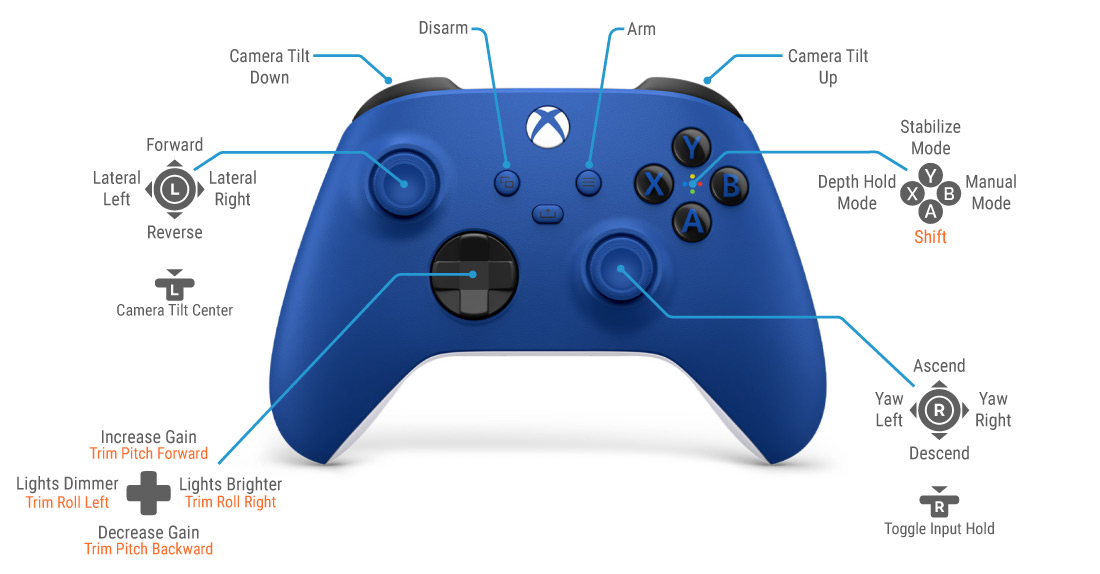
\includegraphics[width=0.6\textwidth]{example.png}
        \caption{Exemple d'image.}
        \label{fig:example}
    \end{figure}
    
    % Section 4
    \section{Conclusion}
    Vous pouvez conclure ici et mentionner les prochaines étapes ou vos observations finales.
    
    % Références
    \begin{thebibliography}{9}
    
    \bibitem{example}
    Auteur, Titre de l'ouvrage, \textit{Éditeur}, Année.
    
    \end{thebibliography}
    
    \end{document}
    
a^2 + b^2 &= c^2 \\
f(x) &= \int_a^b g(x) \, dx
\end{align}

% Section 3
\section{Inclusion d'images}
Vous pouvez inclure des images comme suit (l'image doit être dans le même dossier que le fichier .tex) :

\begin{figure}[h!]
    \centering
    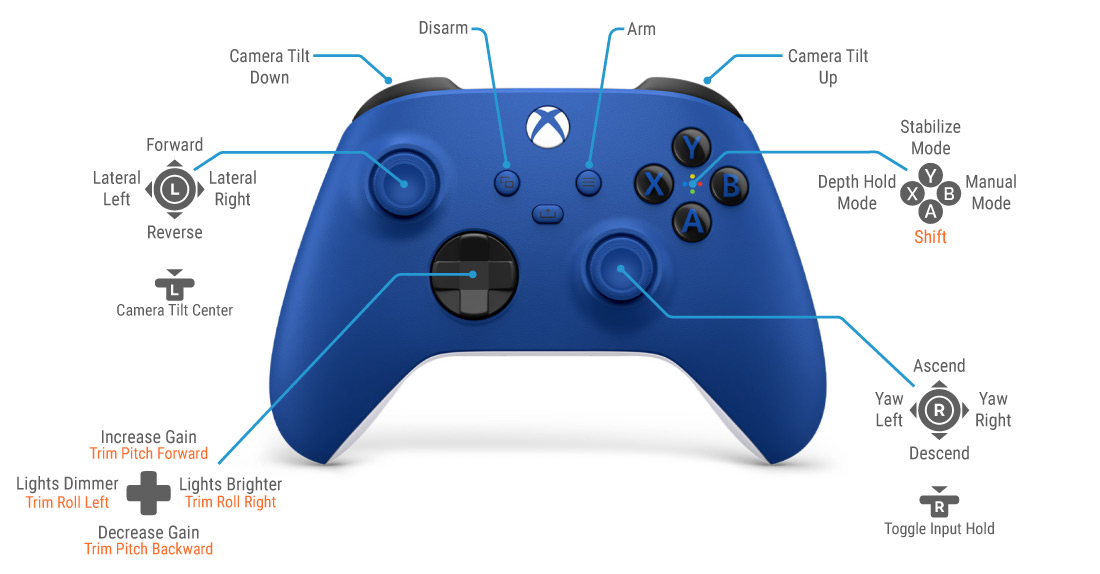
\includegraphics[width=0.6\textwidth]{example.png}
    \caption{Exemple d'image.}
    \label{fig:example}
\end{figure}

% Section 4
\section{Conclusion}
Vous pouvez conclure ici et mentionner les prochaines étapes ou vos observations finales.

% Références
\begin{thebibliography}{9}

\bibitem{example}
Auteur, Titre de l'ouvrage, \textit{Éditeur}, Année.

\end{thebibliography}

\end{document}
